\section{Ejercicio 5}

Implementado el Scheduler Round-Robin, se desea analizar ciertos parámetros de calidad del scheduler comparando los mismos para un quantum de 2, 10 y 50 ciclos.
El lote de tareas para la prueba consiste en el siguiente:

\begin{verbatim}
*3 TaskCPU 50 
*2 TaskConsola 5 3 3
\end{verbatim}

Que especifica tres tareas con uso de CPU durante 50 ciclos y 2 tareas que realizan 5 llamadas bloqueantes con duracion de 3 ciclos cada una.\\

Los parámetros de calidad a analizar son: latencia, waiting time y tiempo total de ejecución, siendo la latencia el tiempo que la tarea pasa en estado ''listo'' hasta que comienza su ejecución, el waiting time el tiempo que pasa una tarea sin ejecutar desde el momento que está en estado ''listo'' hasta que termina su ejecución, y el tiempo total de ejecución el tiempo que toma la tarea desde que está en estado ''listo'' hasta que cumple con su ejecución.

\begin{figure}[h]
  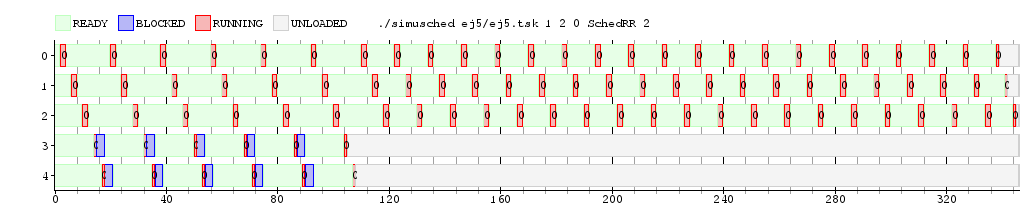
\includegraphics[width=\textwidth]{../ej5/ej5RR1202.png}
  \caption{Tareas con quantum 2.}
  \label{fig:quant2}
\end{figure}


\begin{figure}[h]
  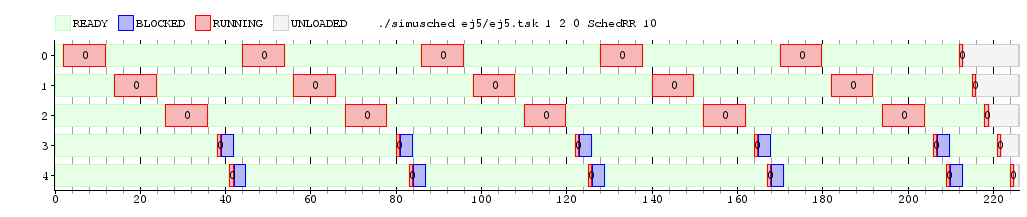
\includegraphics[width=\textwidth]{../ej5/ej5RR12010.png}
  \caption{Tareas con quantum 10.}
  \label{fig:quant10}
\end{figure}


\begin{figure}[h]
  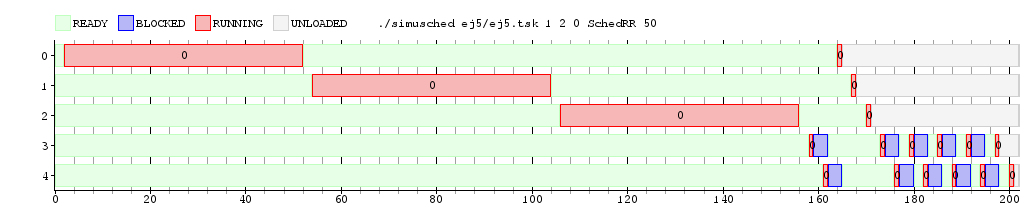
\includegraphics[width=\textwidth]{../ej5/ej5RR12050.png}
  \caption{Tareas con quantum 50.}
  \label{fig:quant50}
\end{figure}


 \begin{table}[h!]
 	\begin{center}
 		\caption{Parámetros de calidad para el sceduler round robin: SchedRR.}
 		\label{tab:table1}
 		\begin{tabular}{|l|c|c|c|c|c|}
 			\hline
 			& Tarea & Latencia & Waiting time & Total ejecución & Ratio (Espera/total) \\
 			\hline
 			\hline
 			\multirow{6}{*}{Quantum = 2}
 			& 0 & 2 & 288 & 339 & 0.85\\ \cline{2-6}
 			& 1 & 6 & 291 & 342 & 0.85 \\ \cline{2-6}
 			& 2 & 10 & 294 & 345 & 0.85 \\ \cline{2-6}
 			& 3 & 14 & 99 & 105 & 0.94 \\ \cline{2-6}
 			& 4 & 17 & 102 & 108 & 0.94 \\ \cline{2-6}
 			& Avg & 9.8 & 214.8 & 227.8 & 0.89 \\
 			\hline
 			\hline
 			\multirow{6}{*}{Quantum = 10}
 			& 0 & 2 & 162 & 213 & 0.76 \\ \cline{2-6}
 			& 1 & 14 & 165 & 216 & 0.76 \\ \cline{2-6}
			& 2 & 26 & 168 & 219 & 0.76 \\ \cline{2-6}
 			& 3 & 38 & 216 & 222 & 0.97 \\ \cline{2-6}
 			& 4 & 41 & 219 & 225 & 0.97 \\ \cline{2-6}
 			& Avg & 24.2 & 186 & 219 & 0.84 \\
 			\hline
 			\hline
 			\multirow{6}{*}{Quantum = 50}
 			& 0 & 2 & 114 & 165 & 0.69 \\ \cline{2-6}
 			& 1 & 54 & 117 & 168 & 0.69 \\ \cline{2-6}
			& 2 & 106 & 120 & 171 & 0.70\\ \cline{2-6}
 			& 3 & 158 & 192 & 198 & 0.97 \\ \cline{2-6}
 			& 4 & 161 & 195 & 201 & 0.97 \\ \cline{2-6}
 			& Avg & 96.2 & 147.6 & 180.6 & 0.80 \\
 			\hline
 		\end{tabular}
 	\end{center}
 \end{table}

Como puede verse en la tabla \ref{tab:table1}, la latencia es menor cuando el quantum es 2 y va subiendo a medida que sube el quantum, esto sucede dado que el scheduler round robin cuando agota su quantum desaloja a la tarea en ejecución y toma una nueva dentro de la cola de tareas que tiene definida. A menor quantum más se apega el scheduler al concepto de time-sharing mientras que a mayor quantum más tienen que esperar las tareas encoladas para empezar su ejecución.

En cuanto a waiting time y tiempo total de ejecución (que están íntimamente relacionados dado que el waiting time es la diferencia entre el tiempo total de ejecución y el tiempo que cada tarea posee el uso de los recursos de CPU), ambos parámetros son menores en promedio mientras mayor es el quantum otorgado a cada tarea. Esto sucede debido a que hay menor cantidad de cambios de contexto mientras más grande es el quantum otorgado a cada tarea. 
Sin embargo el promedio no es totalmente significativo dado que depende fuertemente del tipo y naturaleza de tareas que se ejecutan. Puede verse, por ejemplo, que si bien las tareas que hacen consumo intensivo de CPU mejoran sensiblemente sus parámetros mientras que las tareas que utilizan llamadas bloqueantes se ven afectadas negativamente.

Si tomamos como parámetro de ''justicia'' de un scheduler que sean favorecidos los procesos que menor cantidad de CPU toman, podemos concluir que es más justo un quantum menor, aunque debido al costo de cambio de contexto el cálculo a efectuar debe ser cuidadoso para no desperdiciar demasiado tiempo en el mismo. Se debe tener en cuenta que los valores tomados son basados en lotes de tareas conocidos y en un sistema interactivo hay mayor variabilidad en la naturaleza de las mismas.

\clearpage   %con esto todo se arregla!!!!
